\part{Element Buffer}
\frame{\partpage}

\begin{frame}{Element Buffer}
	\begin{itemize}
		\pause\item If we look at the cube sample, we are sending 36 vertices
		\pause\item This is a bit wasteful considering that some of these vertices are duplicates
		\pause\item We can use an \textbf{Element Buffer} to optimise our drawing
		\pause\item An Element Buffer holds an integer which is an offset into a Vertex Buffer
	\end{itemize}
\end{frame}

\begin{frame}{Creating \& Using Element Buffer}
	\begin{center}
		Live Coding
	\end{center}
\end{frame}

\begin{frame}{Exercise 1 - Let's draw a square!}
\begin{center}
	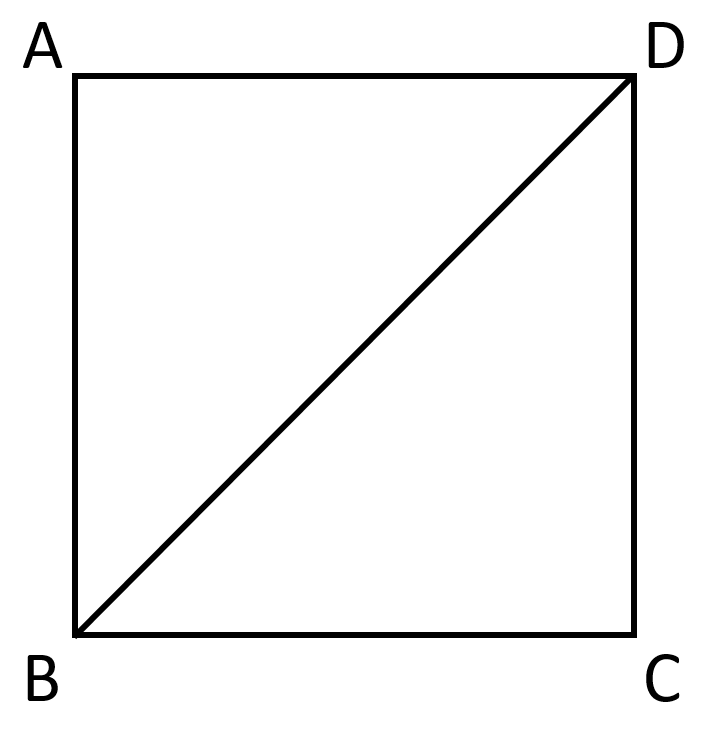
\includegraphics[height=0.8\textheight]{square_vertices}
\end{center}
\end{frame}

\begin{frame}{Exercise 2 - Let's draw a cube!}
	\begin{center}
	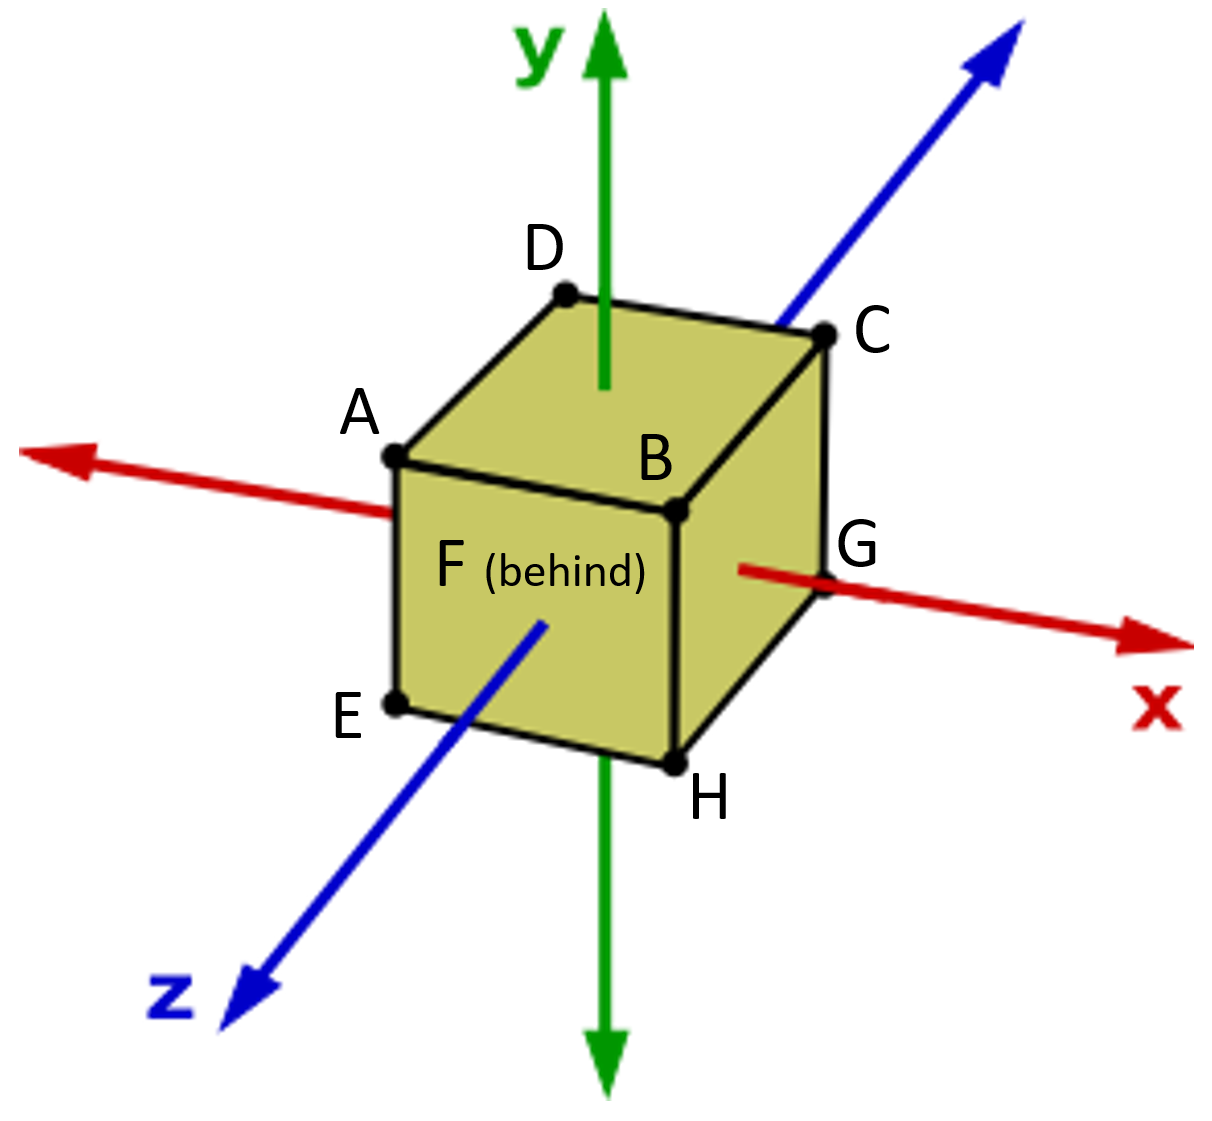
\includegraphics[height=0.8\textheight]{cube_vertices}
	\end{center}
\end{frame}

\begin{frame}{Exercise 3 - Element Buffer}
	\begin{itemize}
		\item Create a cube using an Element Buffer
		\item Create a function which fills a Vertex Buffer and Element Buffer for drawing a Sphere
	\end{itemize}
\end{frame}

\begin{frame}{Further Reading - Interleaved Vertices}
	\begin{itemize}
		\item iOS Development Docs - \url{https://developer.apple.com/library/content/documentation/3DDrawing/Conceptual/OpenGLES_ProgrammingGuide/TechniquesforWorkingwithVertexData/TechniquesforWorkingwithVertexData.html}
		\item To interleave or not to interleave - \url{https://anteru.net/blog/2016/02/14/3119/index.html}
		\item Vertex Specification Best Practices - \url{https://www.khronos.org/opengl/wiki/Vertex_Specification_Best_Practices}
	\end{itemize}
\end{frame}

\begin{frame}{Further Reading - Element Buffer}
	\begin{itemize}
		\item VBO indexing - \url{http://www.opengl-tutorial.org/intermediate-tutorials/tutorial-9-vbo-indexing/}
		\item Element Buffer - \url{https://goharsha.com/lwjgl-tutorial-series/element-buffer-objects/}
	\end{itemize}
\end{frame}


